% Options for packages loaded elsewhere
\PassOptionsToPackage{unicode}{hyperref}
\PassOptionsToPackage{hyphens}{url}
%
\documentclass[
]{book}
\usepackage{amsmath,amssymb}
\usepackage{lmodern}
\usepackage{ifxetex,ifluatex}
\ifnum 0\ifxetex 1\fi\ifluatex 1\fi=0 % if pdftex
  \usepackage[T1]{fontenc}
  \usepackage[utf8]{inputenc}
  \usepackage{textcomp} % provide euro and other symbols
\else % if luatex or xetex
  \usepackage{unicode-math}
  \defaultfontfeatures{Scale=MatchLowercase}
  \defaultfontfeatures[\rmfamily]{Ligatures=TeX,Scale=1}
\fi
% Use upquote if available, for straight quotes in verbatim environments
\IfFileExists{upquote.sty}{\usepackage{upquote}}{}
\IfFileExists{microtype.sty}{% use microtype if available
  \usepackage[]{microtype}
  \UseMicrotypeSet[protrusion]{basicmath} % disable protrusion for tt fonts
}{}
\makeatletter
\@ifundefined{KOMAClassName}{% if non-KOMA class
  \IfFileExists{parskip.sty}{%
    \usepackage{parskip}
  }{% else
    \setlength{\parindent}{0pt}
    \setlength{\parskip}{6pt plus 2pt minus 1pt}}
}{% if KOMA class
  \KOMAoptions{parskip=half}}
\makeatother
\usepackage{xcolor}
\IfFileExists{xurl.sty}{\usepackage{xurl}}{} % add URL line breaks if available
\IfFileExists{bookmark.sty}{\usepackage{bookmark}}{\usepackage{hyperref}}
\hypersetup{
  pdftitle={Galaxy Workflow for RNAseq},
  pdfauthor={David Innes},
  hidelinks,
  pdfcreator={LaTeX via pandoc}}
\urlstyle{same} % disable monospaced font for URLs
\usepackage{color}
\usepackage{fancyvrb}
\newcommand{\VerbBar}{|}
\newcommand{\VERB}{\Verb[commandchars=\\\{\}]}
\DefineVerbatimEnvironment{Highlighting}{Verbatim}{commandchars=\\\{\}}
% Add ',fontsize=\small' for more characters per line
\usepackage{framed}
\definecolor{shadecolor}{RGB}{248,248,248}
\newenvironment{Shaded}{\begin{snugshade}}{\end{snugshade}}
\newcommand{\AlertTok}[1]{\textcolor[rgb]{0.94,0.16,0.16}{#1}}
\newcommand{\AnnotationTok}[1]{\textcolor[rgb]{0.56,0.35,0.01}{\textbf{\textit{#1}}}}
\newcommand{\AttributeTok}[1]{\textcolor[rgb]{0.77,0.63,0.00}{#1}}
\newcommand{\BaseNTok}[1]{\textcolor[rgb]{0.00,0.00,0.81}{#1}}
\newcommand{\BuiltInTok}[1]{#1}
\newcommand{\CharTok}[1]{\textcolor[rgb]{0.31,0.60,0.02}{#1}}
\newcommand{\CommentTok}[1]{\textcolor[rgb]{0.56,0.35,0.01}{\textit{#1}}}
\newcommand{\CommentVarTok}[1]{\textcolor[rgb]{0.56,0.35,0.01}{\textbf{\textit{#1}}}}
\newcommand{\ConstantTok}[1]{\textcolor[rgb]{0.00,0.00,0.00}{#1}}
\newcommand{\ControlFlowTok}[1]{\textcolor[rgb]{0.13,0.29,0.53}{\textbf{#1}}}
\newcommand{\DataTypeTok}[1]{\textcolor[rgb]{0.13,0.29,0.53}{#1}}
\newcommand{\DecValTok}[1]{\textcolor[rgb]{0.00,0.00,0.81}{#1}}
\newcommand{\DocumentationTok}[1]{\textcolor[rgb]{0.56,0.35,0.01}{\textbf{\textit{#1}}}}
\newcommand{\ErrorTok}[1]{\textcolor[rgb]{0.64,0.00,0.00}{\textbf{#1}}}
\newcommand{\ExtensionTok}[1]{#1}
\newcommand{\FloatTok}[1]{\textcolor[rgb]{0.00,0.00,0.81}{#1}}
\newcommand{\FunctionTok}[1]{\textcolor[rgb]{0.00,0.00,0.00}{#1}}
\newcommand{\ImportTok}[1]{#1}
\newcommand{\InformationTok}[1]{\textcolor[rgb]{0.56,0.35,0.01}{\textbf{\textit{#1}}}}
\newcommand{\KeywordTok}[1]{\textcolor[rgb]{0.13,0.29,0.53}{\textbf{#1}}}
\newcommand{\NormalTok}[1]{#1}
\newcommand{\OperatorTok}[1]{\textcolor[rgb]{0.81,0.36,0.00}{\textbf{#1}}}
\newcommand{\OtherTok}[1]{\textcolor[rgb]{0.56,0.35,0.01}{#1}}
\newcommand{\PreprocessorTok}[1]{\textcolor[rgb]{0.56,0.35,0.01}{\textit{#1}}}
\newcommand{\RegionMarkerTok}[1]{#1}
\newcommand{\SpecialCharTok}[1]{\textcolor[rgb]{0.00,0.00,0.00}{#1}}
\newcommand{\SpecialStringTok}[1]{\textcolor[rgb]{0.31,0.60,0.02}{#1}}
\newcommand{\StringTok}[1]{\textcolor[rgb]{0.31,0.60,0.02}{#1}}
\newcommand{\VariableTok}[1]{\textcolor[rgb]{0.00,0.00,0.00}{#1}}
\newcommand{\VerbatimStringTok}[1]{\textcolor[rgb]{0.31,0.60,0.02}{#1}}
\newcommand{\WarningTok}[1]{\textcolor[rgb]{0.56,0.35,0.01}{\textbf{\textit{#1}}}}
\usepackage{longtable,booktabs,array}
\usepackage{calc} % for calculating minipage widths
% Correct order of tables after \paragraph or \subparagraph
\usepackage{etoolbox}
\makeatletter
\patchcmd\longtable{\par}{\if@noskipsec\mbox{}\fi\par}{}{}
\makeatother
% Allow footnotes in longtable head/foot
\IfFileExists{footnotehyper.sty}{\usepackage{footnotehyper}}{\usepackage{footnote}}
\makesavenoteenv{longtable}
\usepackage{graphicx}
\makeatletter
\def\maxwidth{\ifdim\Gin@nat@width>\linewidth\linewidth\else\Gin@nat@width\fi}
\def\maxheight{\ifdim\Gin@nat@height>\textheight\textheight\else\Gin@nat@height\fi}
\makeatother
% Scale images if necessary, so that they will not overflow the page
% margins by default, and it is still possible to overwrite the defaults
% using explicit options in \includegraphics[width, height, ...]{}
\setkeys{Gin}{width=\maxwidth,height=\maxheight,keepaspectratio}
% Set default figure placement to htbp
\makeatletter
\def\fps@figure{htbp}
\makeatother
\setlength{\emergencystretch}{3em} % prevent overfull lines
\providecommand{\tightlist}{%
  \setlength{\itemsep}{0pt}\setlength{\parskip}{0pt}}
\setcounter{secnumdepth}{5}
\usepackage{booktabs}
\ifluatex
  \usepackage{selnolig}  % disable illegal ligatures
\fi
\usepackage[]{natbib}
\bibliographystyle{plainnat}

\title{Galaxy Workflow for RNAseq}
\author{David Innes}
\date{2022-01-05}

\begin{document}
\maketitle

{
\setcounter{tocdepth}{1}
\tableofcontents
}
\hypertarget{about}{%
\chapter{About}\label{about}}

These instructions show how to use pre-made workflows on \url{usegalaxy.org.au}
to analyse single stranded RNAseq files outputted from an Illumina system.

This assumes some familularity with Galaxy, but also aims to help beginners complete this specific use-case. Other tutorials are more generalised and are better equipped to help users learn each stop of RNAseq pipelines.

It is broken into 2 workflows. A workflow is a set of tools on galaxy organised together to do certain tasks. These workflows are shareable and are included here. Therefore many steps are automated and not discussed, but the details can be viewed when exploring these workflows within Galaxy.

\hypertarget{workflow-step-1}{%
\section*{Workflow Step 1}\label{workflow-step-1}}
\addcontentsline{toc}{section}{Workflow Step 1}

The first workflow is designed to rename files, run quality check for each file and join any files together that are from the same sample (see \ref{multiple-lane-files}). It also calculates some other values required for Step 2, such as the length of bp of the transcripts.

Once the output is checked (FastQC via a MultiQC report), the concatenated files can be used as input to Step 2.

\hypertarget{workflow-step-2}{%
\section*{Workflow Step 2}\label{workflow-step-2}}
\addcontentsline{toc}{section}{Workflow Step 2}

This workflow re-runs fastQC with the input files, and uses trimmomatic, RNA STAR Aligner and featureCounts to produce the required outputs for downstream analysis. It also reports each step to MultiQC webpage.

\hypertarget{user-profile}{%
\section*{User profile}\label{user-profile}}
\addcontentsline{toc}{section}{User profile}

You will need to be signed in to complete this analysis. Make sure you use university email address when setting up profile. Registered users with an Australian research institute are allocated 600GB, otherwise only 100GB is allocated.

\hypertarget{upload-and-prepare-data}{%
\chapter{Upload and Prepare Data}\label{upload-and-prepare-data}}

\hypertarget{import-fastq-files}{%
\section{Import fastq files}\label{import-fastq-files}}

\hypertarget{upload}{%
\subsection{Upload}\label{upload}}

Firstly we upload the files to the Galaxy History. Follow figures below.

\begin{figure}

{\centering 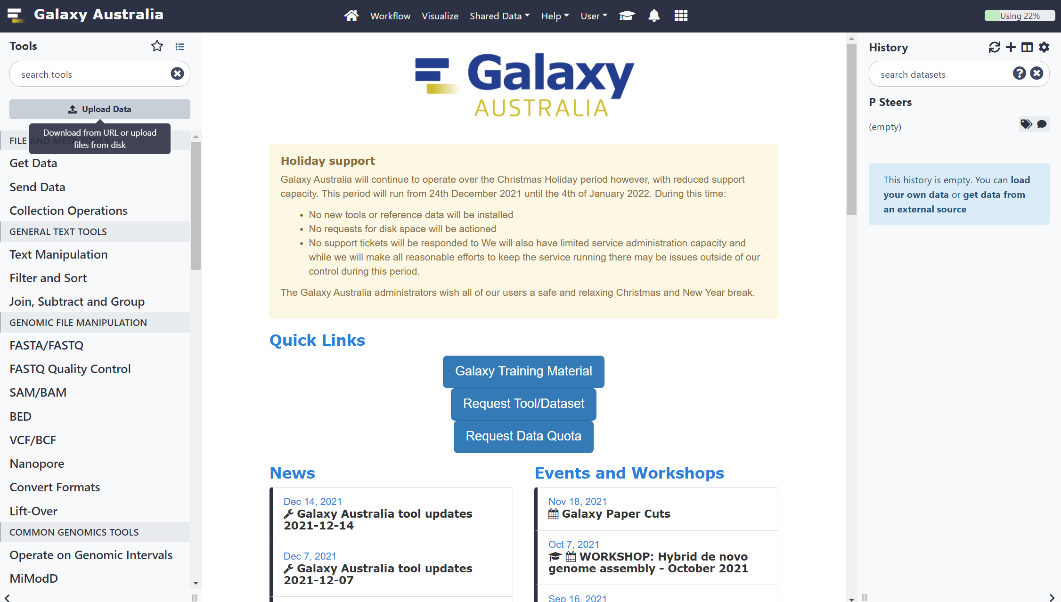
\includegraphics[width=1\linewidth]{images/image001} 

}

\caption{Click Upload Data button}\label{fig:chunk1}
\end{figure}

\begin{figure}

{\centering 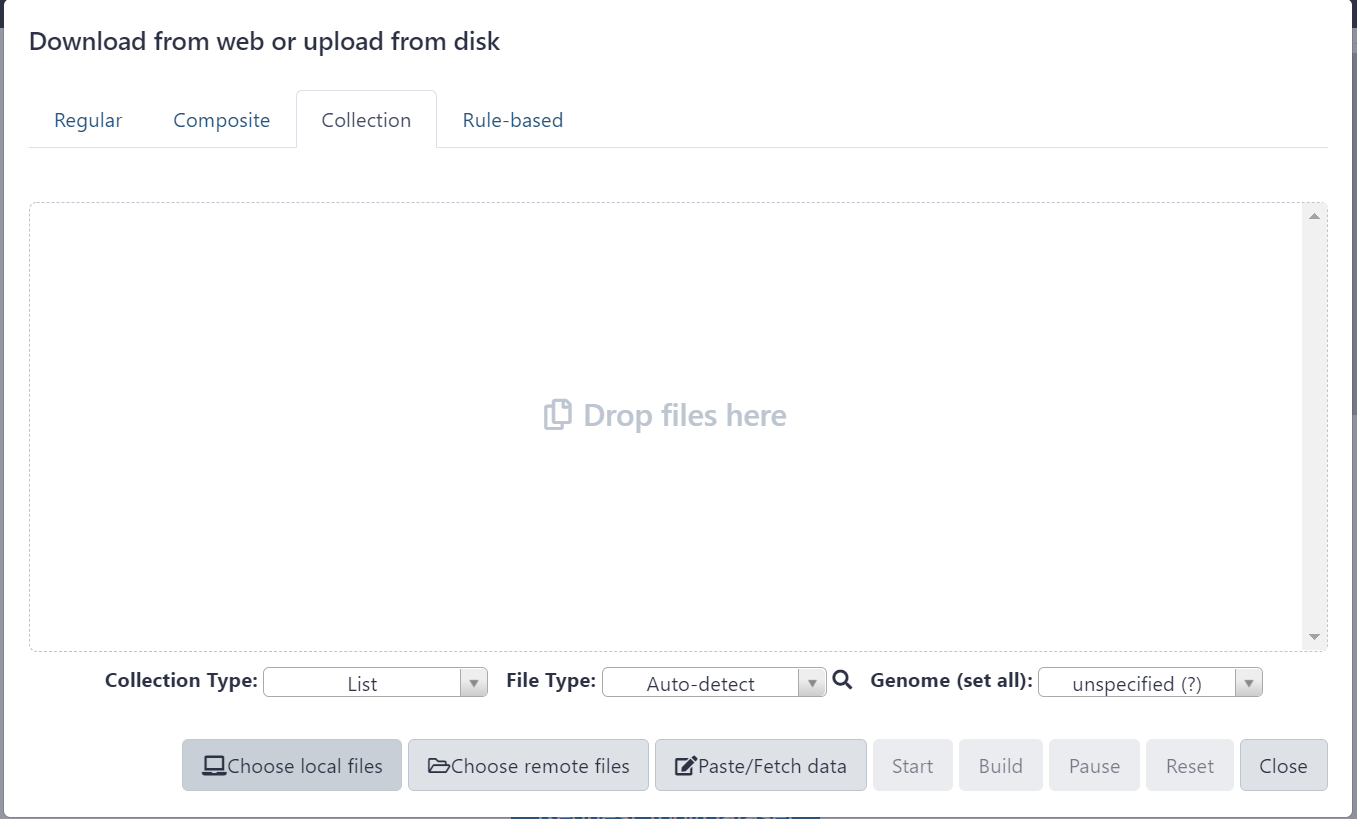
\includegraphics[width=1\linewidth]{images/image002} 

}

\caption{Select ‘Collection’ from the top ribbon and click ‘Choose local files’ button}\label{fig:chunk2}
\end{figure}

\begin{figure}

{\centering 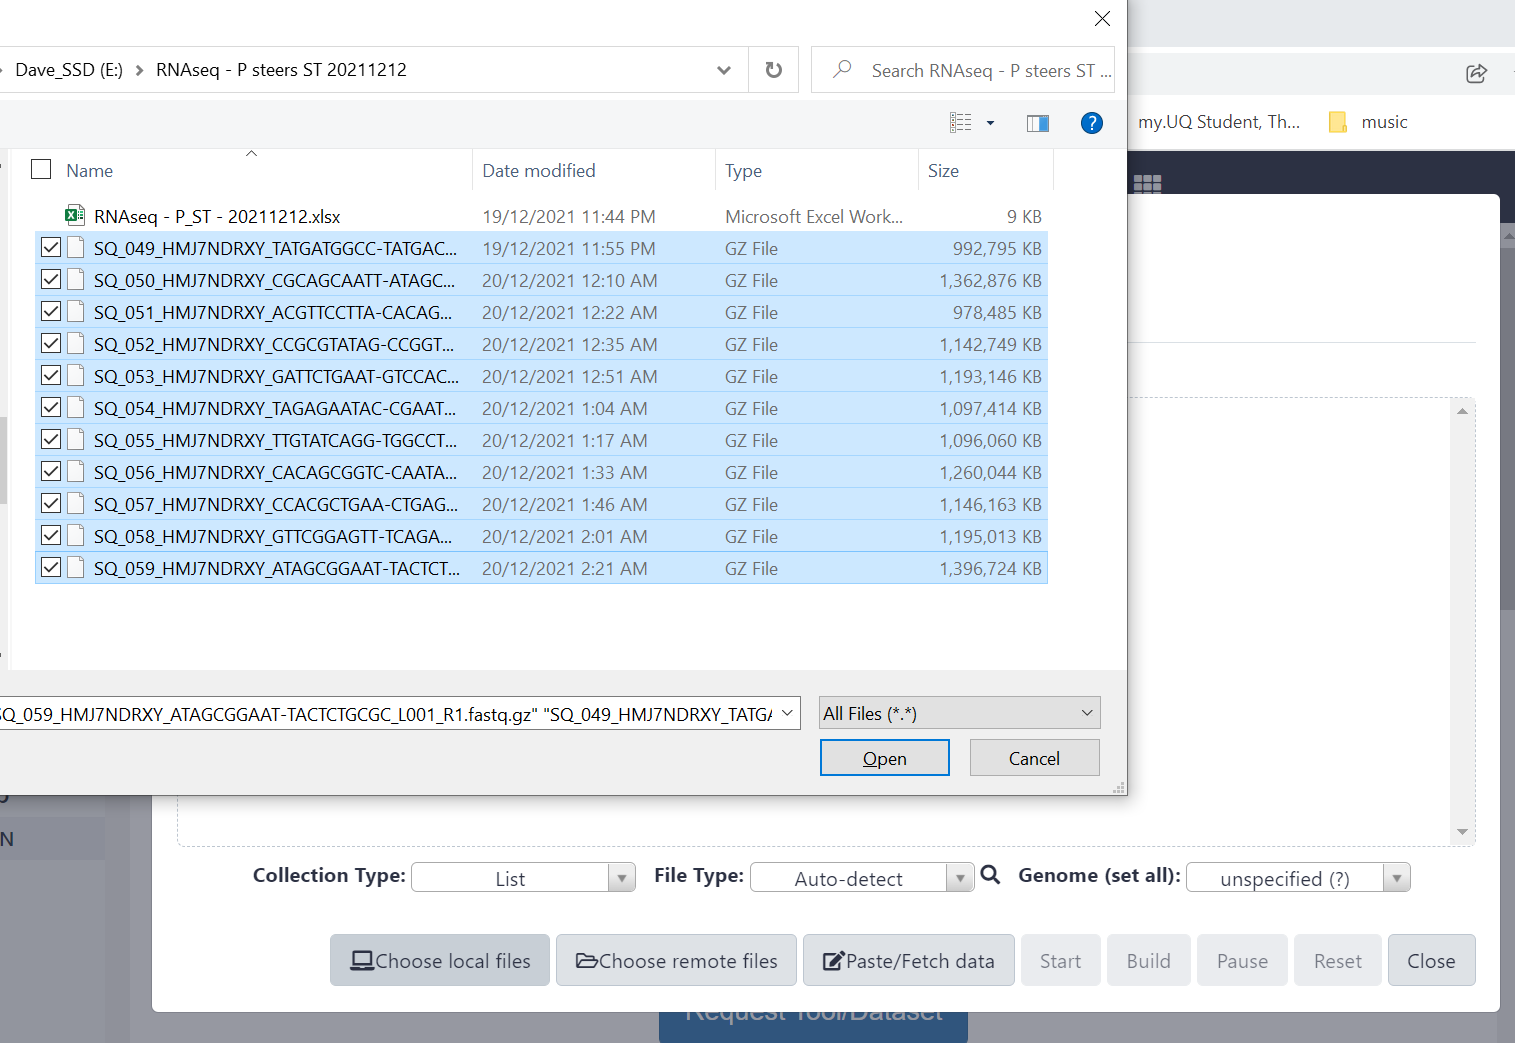
\includegraphics[width=1\linewidth]{images/image003} 

}

\caption{Navigate to the files to upload and highlight them all using Shift or Ctrl keys to help, then click ‘Open’}\label{fig:chunk3}
\end{figure}

\begin{figure}

{\centering 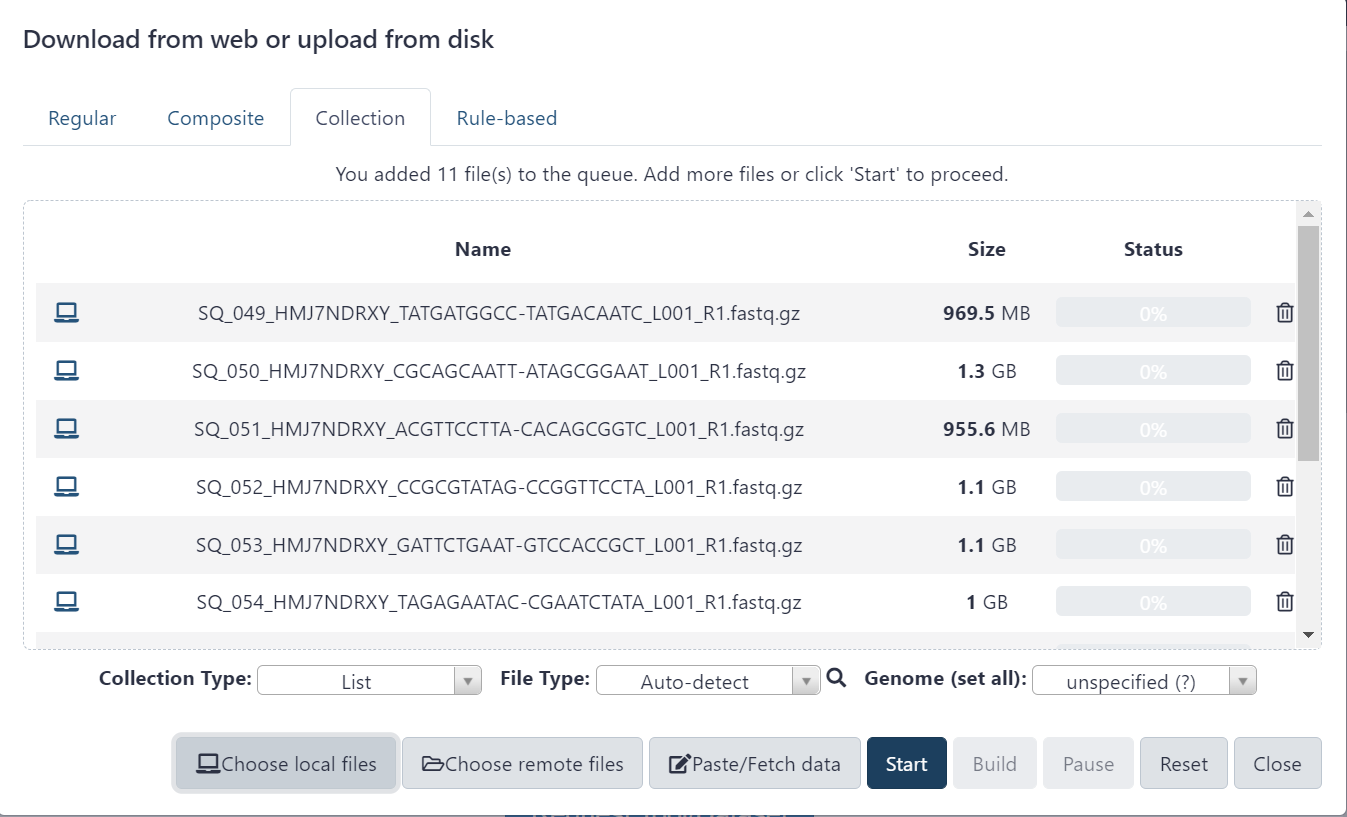
\includegraphics[width=1\linewidth]{images/image004} 

}

\caption{Click ‘Start’ button to begin uploading files. Keep this website open until it is finished.}\label{fig:chunk4}
\end{figure}

\hypertarget{add-files-to-a-collection}{%
\subsection{Add files to a `collection'}\label{add-files-to-a-collection}}

Once the files have uploaded they will appear in the History pane. Next, we add them to a `collection', which is basically just a list of files. It allows all files to be parsed through a workflow one by one. For example, if a tool was used on a collection, then each item in the list/collection would invoke its own job while all output is kept within a collection in the history.

\begin{figure}

{\centering 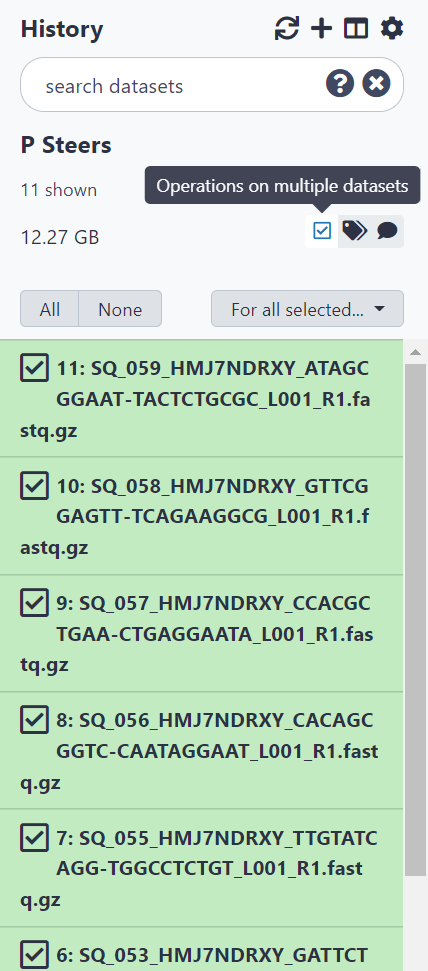
\includegraphics[width=5.94in]{images/image005} 

}

\caption{Select ‘Operations on multiple datasets’ then select all items to add to collection}\label{fig:chunk5}
\end{figure}

\begin{figure}

{\centering 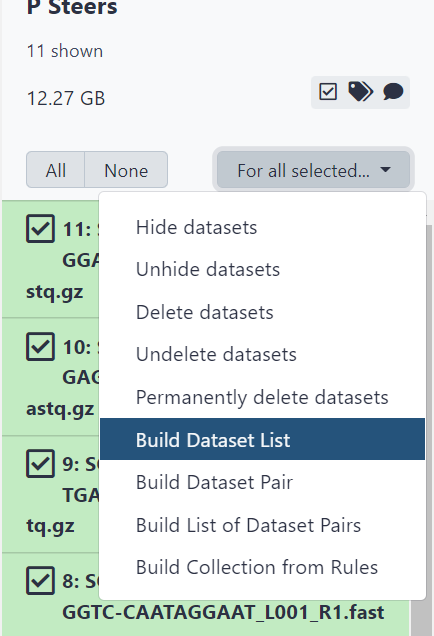
\includegraphics[width=6.03in]{images/image006} 

}

\caption{Click ‘For all selected’ then 'Build dataset list'}\label{fig:chunk6}
\end{figure}

\begin{figure}

{\centering 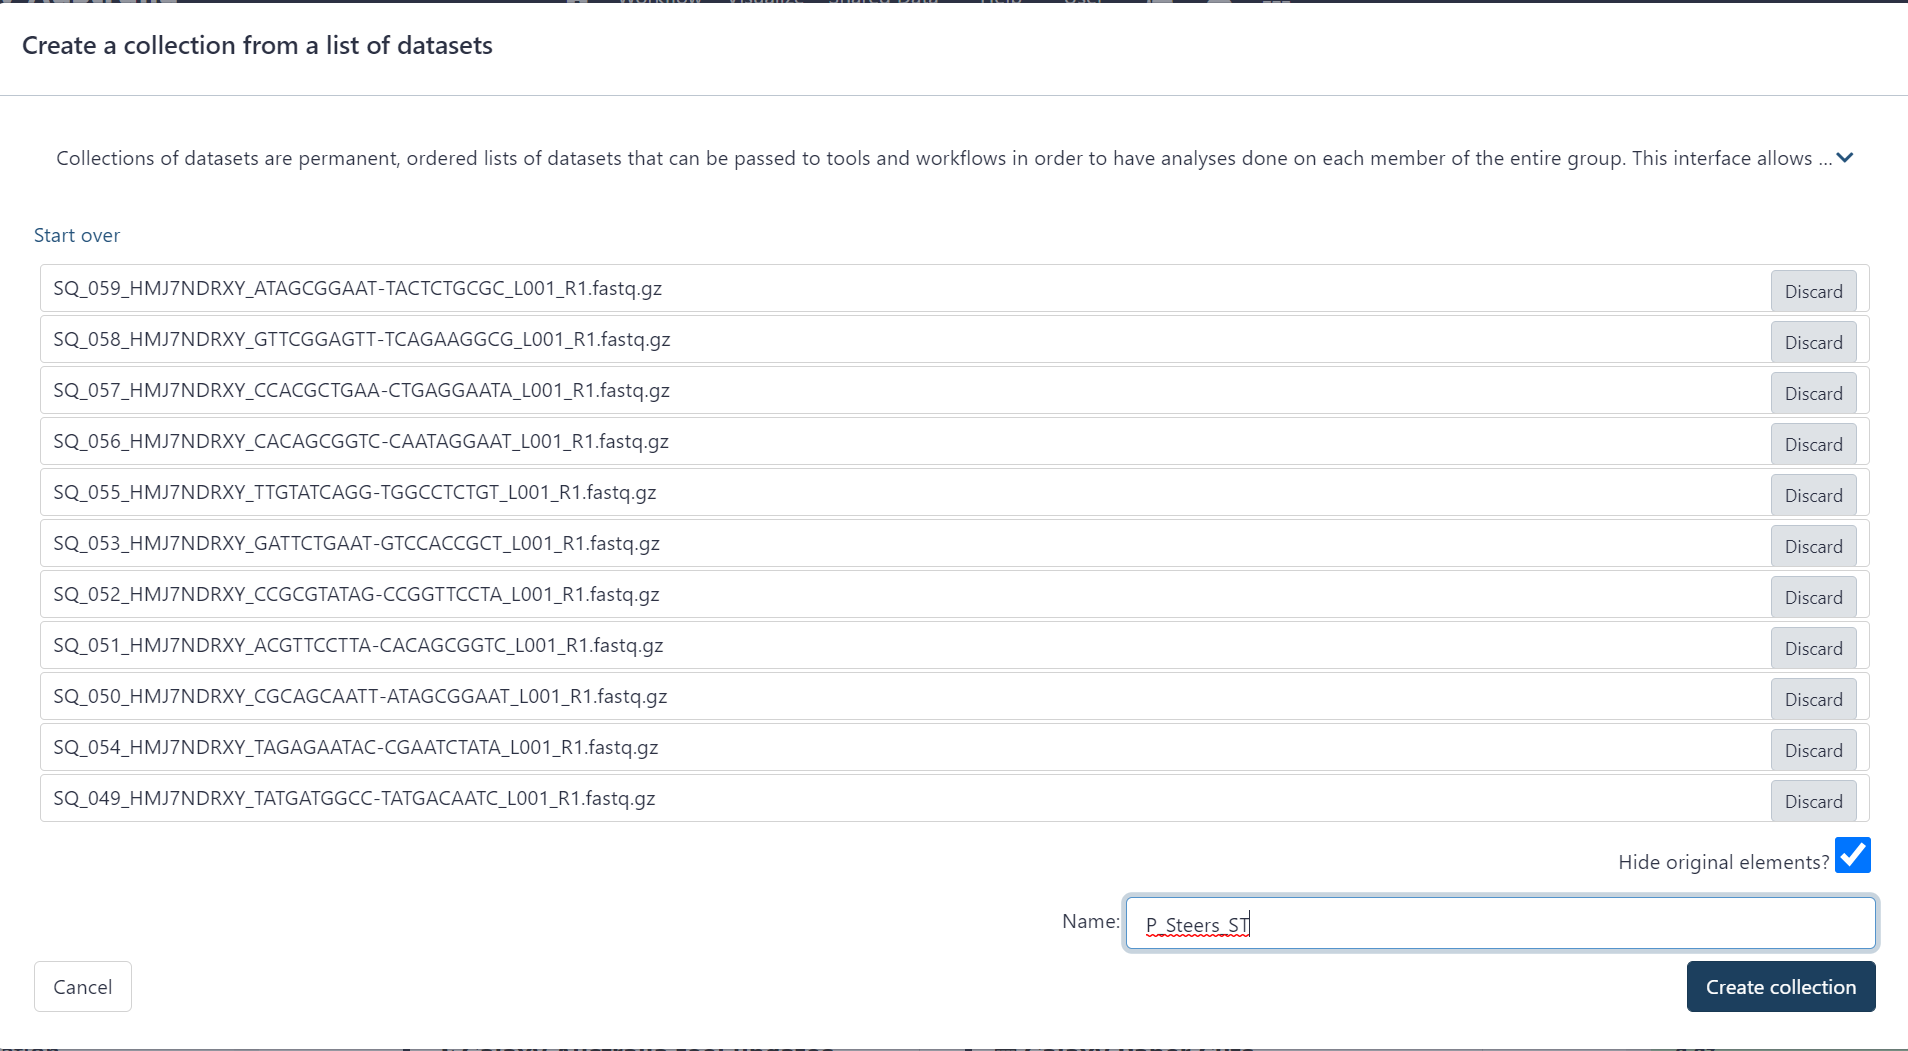
\includegraphics[width=1\linewidth]{images/image007} 

}

\caption{Type a name for the list and click ‘Create collection’ button}\label{fig:chunk7}
\end{figure}

\begin{figure}

{\centering 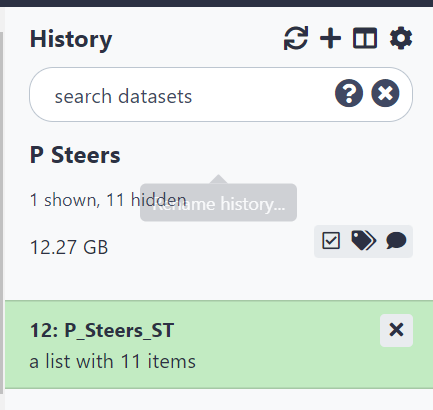
\includegraphics[width=6.01in]{images/image008} 

}

\caption{All files should now be in a collection in the History pane.}\label{fig:chunk8}
\end{figure}

\hypertarget{rename-files}{%
\section{Rename Files}\label{rename-files}}

This step renames the files to more meaningful and user friendly names.

To do this, a new file is imported with the old names and the new names. This should be a tab delimited .txt file with 2 columns of data.

The 1st column has original name (which is likely to be filename) and the 2nd column has new names. E.g. original filename might be \texttt{SQ\_049\_HMJ7NDRXY\_TATGATGGCC-TATGACAATC\_L001\_R1.fastq.gz} whereas new name could be changed to include treatment information such as \texttt{ST\_811\_P5\_L001}.
It is important that the "\_L" number is included at the end, even if there is not multiple lanes per sample. This will be dealt with by the ``Step 1'' workflow. See section \ref{rename-note}.

Use the `upload data' feature of galaxy to import the .txt file to to the History. It should look something like \ref{fig:example-rename}.

\begin{figure}

{\centering 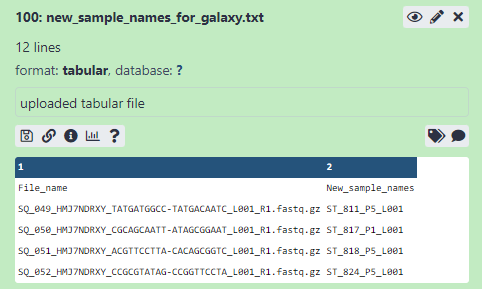
\includegraphics[width=1\linewidth]{images/image009} 

}

\caption{Example of text file imported to History with original and new filenames}\label{fig:example-rename}
\end{figure}

This .txt file can be made in Excel, or it can be done much quicker using a simple R script. The following is an example script:

\begin{Shaded}
\begin{Highlighting}[]
\CommentTok{\# list file names and create table with new file names for use in galaxy\textquotesingle{}s "Relabel list identifiers" tool}
\FunctionTok{library}\NormalTok{(tidyverse)}
\FunctionTok{library}\NormalTok{(data.table)}

\CommentTok{\#list the names of the fastq files in the working directory}
\NormalTok{file\_list }\OtherTok{\textless{}{-}} \FunctionTok{list.files}\NormalTok{(}\AttributeTok{path =} \StringTok{"E:/RNAseq {-} P steers ST 20211212/"}\NormalTok{, }\AttributeTok{pattern =} \StringTok{".fastq"}\NormalTok{)}

\CommentTok{\#list .csv files to select the .csv file that contains sample information}
\NormalTok{files\_csv }\OtherTok{\textless{}{-}} \FunctionTok{list.files}\NormalTok{(}\AttributeTok{path =} \StringTok{"E:/RNAseq {-} P steers ST 20211212/"}\NormalTok{, }\AttributeTok{pattern =} \StringTok{".csv"}\NormalTok{)}

\CommentTok{\#selects the correct .csv file, in this case there is only 1 file anyway, but the correct file can be selected by entering it\textquotesingle{}s number in the list in the []}
\NormalTok{selected\_file }\OtherTok{\textless{}{-}}\NormalTok{ files\_csv[}\DecValTok{1}\NormalTok{]}
\FunctionTok{message}\NormalTok{(}\FunctionTok{paste}\NormalTok{(}\StringTok{"Selected file {-}"}\NormalTok{, selected\_file))}

\CommentTok{\#import the selected file, making sure no columns have the same name}
\NormalTok{sample\_IDs }\OtherTok{\textless{}{-}} \FunctionTok{fread}\NormalTok{(}\AttributeTok{file =} \FunctionTok{paste0}\NormalTok{(}\StringTok{"E:/RNAseq {-} P steers ST 20211212/"}\NormalTok{,selected\_file)) }\SpecialCharTok{\%\textgreater{}\%} 
  \FunctionTok{as\_tibble}\NormalTok{(}\AttributeTok{.name\_repair =} \StringTok{"unique"}\NormalTok{) }\SpecialCharTok{\%\textgreater{}\%} 
  \FunctionTok{mutate}\NormalTok{(}\StringTok{\textasciigrave{}}\AttributeTok{Steer ID}\StringTok{\textasciigrave{}} \OtherTok{=} \FunctionTok{as.character}\NormalTok{(}\StringTok{\textasciigrave{}}\AttributeTok{Steer ID}\StringTok{\textasciigrave{}}\NormalTok{)) }


\CommentTok{\#As the file names have a set structure, it can be split by the \_ character}
\NormalTok{df\_file\_names\_split }\OtherTok{\textless{}{-}} \FunctionTok{str\_split}\NormalTok{(file\_list, }\AttributeTok{pattern =} \StringTok{"\_"}\NormalTok{, }\AttributeTok{simplify =} \ConstantTok{TRUE}\NormalTok{) }\SpecialCharTok{\%\textgreater{}\%} \FunctionTok{as.data.frame}\NormalTok{()}

\CommentTok{\#In this example, the \textquotesingle{}key\textquotesingle{} column is the RNAseq\_ID column. So this will be modified to remove the \textquotesingle{}SQ\_\textquotesingle{} from the ID so that it can match.}
\NormalTok{sample\_IDs }\OtherTok{\textless{}{-}} 
\NormalTok{  sample\_IDs }\SpecialCharTok{\%\textgreater{}\%} 
  \FunctionTok{mutate}\NormalTok{(}\AttributeTok{RNAseq\_ID\_2 =} \FunctionTok{str\_remove}\NormalTok{(RNAseq\_ID, }\StringTok{"SQ\_"}\NormalTok{),}
         \AttributeTok{Treatment2 =} \FunctionTok{str\_remove}\NormalTok{(Treatment, }\StringTok{\textquotesingle{}{-}\textquotesingle{}}\NormalTok{))}

\CommentTok{\#join the sampleID annotations to this dataframe, concat required columns for new name}
\NormalTok{new\_names }\OtherTok{\textless{}{-}}\NormalTok{ df\_file\_names\_split }\SpecialCharTok{\%\textgreater{}\%} 
  \FunctionTok{left\_join}\NormalTok{(sample\_IDs, }\AttributeTok{by =} \FunctionTok{c}\NormalTok{(}\StringTok{"V2"} \OtherTok{=} \StringTok{"RNAseq\_ID\_2"}\NormalTok{)) }\SpecialCharTok{\%\textgreater{}\%} 
  \FunctionTok{mutate}\NormalTok{(}\AttributeTok{new\_sample\_names =} \FunctionTok{str\_c}\NormalTok{(}\StringTok{\textasciigrave{}}\AttributeTok{Tissue type}\StringTok{\textasciigrave{}}\NormalTok{,}\StringTok{\textasciigrave{}}\AttributeTok{Steer ID}\StringTok{\textasciigrave{}}\NormalTok{, Treatment2, V5, }\AttributeTok{sep =} \StringTok{"\_"}\NormalTok{)) }\SpecialCharTok{\%\textgreater{}\%} \CommentTok{\#make new names with ID\_Treatmentinfo\_Lane}
\NormalTok{  magrittr}\SpecialCharTok{::}\FunctionTok{use\_series}\NormalTok{(new\_sample\_names) }\CommentTok{\#select only the required column as a list (not a table)}

\CommentTok{\#create new table with only old file names and new names}
\NormalTok{new\_name\_table }\OtherTok{\textless{}{-}}
  \FunctionTok{data.frame}\NormalTok{(}\StringTok{"File\_name"} \OtherTok{=}\NormalTok{ file\_list, }\StringTok{"New\_sample\_names"} \OtherTok{=}\NormalTok{ new\_names)}

\CommentTok{\#export to working directory, as tab delim }
\FunctionTok{fwrite}\NormalTok{(new\_name\_table, }\AttributeTok{file =} \StringTok{"E:/RNAseq {-} P steers ST 20211212/new\_sample\_names\_for\_galaxy.txt"}\NormalTok{, }\AttributeTok{sep =} \StringTok{"}\SpecialCharTok{\textbackslash{}t}\StringTok{"}\NormalTok{)}
\end{Highlighting}
\end{Shaded}

\hypertarget{rename-note}{%
\subsection{A note on multiple lanes}\label{rename-note}}

The output from Illumina sequencing is sometimes provided in multiple files, each corresponding to a `Lane' on the sequencer. It would be easier to ask the lab to provide the output as a single file, which can be computed using the \texttt{-\/-no-lane-splitting} option from Illumina's \texttt{bcl2fastq} program. However, it can also be handled in Galaxy. If there are multiple files, it is best practice to run FastQC on each individual file, as there is a chance that one file could be corrupt or you may identify a bias for one particular `Lane'. If they are ok, then these files can be concatenated together before proceeding with all further steps.

This is described further in \ref{multiple-lane-files}. Make sure the new names generated in \ref{rename-files} have a format that includes "\_L". The protocol relies on there being a `\_L' in the name for it to find the lane number. The rest of the name before the `\_L' should be the same.

E.g. the following three files would be concatenated together by the ``Step 1'' workflow:

\begin{itemize}
\tightlist
\item
  2139\_Stage 2\_Fast\_L008
\item
  2139\_Stage 2\_Fast\_L007
\item
  2139\_Stage 2\_Fast\_L006
\end{itemize}

\hypertarget{import-ensembl-files}{%
\section{Import ENSEMBL files}\label{import-ensembl-files}}

In this step we need to import the required fastq file for sequence alignment and a gtf file for gene annotation.
These can be uploaded directly to Galaxy via a URL. To find the required files, navigate to \url{http://ftp.ensembl.org} in a browser.

For sheep (ovis\_aries) these might be:

\begin{itemize}
\tightlist
\item
  \url{http://ftp.ensembl.org/pub/release-100/fasta/ovis_aries/dna/Ovis_aries.Oar_v3.1.dna.toplevel.fa.gz}
\item
  \url{http://ftp.ensembl.org/pub/release-100/gtf/ovis_aries/Ovis_aries.Oar_v3.1.100.gtf.gz}
\end{itemize}

For cattle (bos\_taurus) these might be:

\begin{itemize}
\tightlist
\item
  \url{http://ftp.ensembl.org/pub/release-100/fasta/bos_taurus/dna/Bos_taurus.ARS-UCD1.2.dna.toplevel.fa.gz}
\item
  \url{http://ftp.ensembl.org/pub/release-100/gtf/bos_taurus/Bos_taurus.ARS-UCD1.2.100.gtf.gz}
\end{itemize}

Note that unmasked files are used here (i.e.~use files without \texttt{\_rm} or \texttt{\_sm}).

To upload these to Galaxy, use the `Paste/Fetch data' button in the `Upload data' dialogue box on Galaxy.

\begin{figure}

{\centering 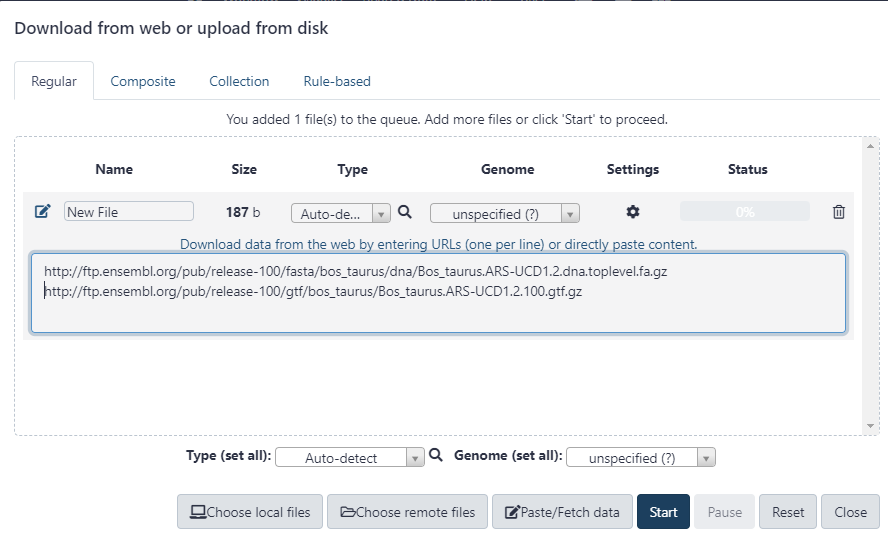
\includegraphics[width=1\linewidth]{images/image_upload_url} 

}

\caption{Paste each URL on a new line to upload directly from ENSEMBL to Galaxy.}\label{fig:paste-url}
\end{figure}

Once executed, 2 new files will appear in the History, each named as the URL entered. This can take some time to finish as they are large files.

\hypertarget{uncompress-.gtf-file}{%
\subsection{Uncompress .gtf file}\label{uncompress-.gtf-file}}

These files are actually .gz files, which means they are compressed. Normally, this is automatically handled by Galaxy but does not currently work for the .gtf file when using it with the \texttt{STAR\ Aligner} in this workflow. Therefore, use the tool \url{https://usegalaxy.org.au/root?tool_id=CONVERTER_gz_to_uncompressed} to uncompress the .gtf file before proceeding.

Once it is uncompressed it may not have the correct file format attributed to it in Galaxy. Fix this by using the auto-detect feature within the Datatypes ribbon of the Edit Attributes section.

\begin{figure}

{\centering 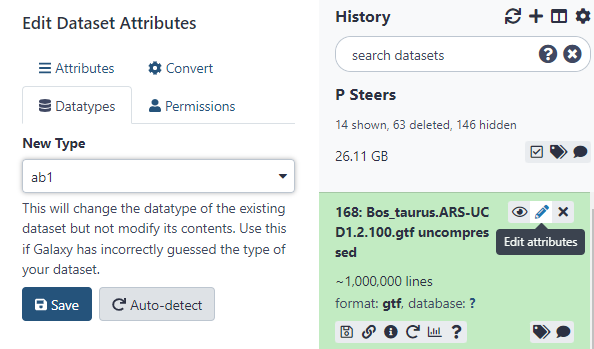
\includegraphics[width=1\linewidth]{images/image_edit_attributes} 

}

\caption{Click 'edit attributes' then navigate to 'Datatypes' to use the Auto-Detect. Otherwise manually set it to .gtf}\label{fig:edit-attributes}
\end{figure}

\hypertarget{step1}{%
\chapter{Workflow - Step 1}\label{step1}}

Once all of the data is uploaded to Galaxy it is time to run/invoke the workflows.
The first workflow is relatively fast compared to Step 2, but is important for QC and to prepare data.

\hypertarget{find-workflow}{%
\section{Find workflow}\label{find-workflow}}

The workflow used here is published at: \url{https://usegalaxy.org.au/u/dave-innes/w/rna-seq-step-1}

This workflow will need to be imported into your personal galaxy profile. Navigate to: \url{https://usegalaxy.org.au/workflows/import}
On this page you will be able to enter the workflow URL above. This will also be required for Step 2.

You can also navigate directly the workflow's URL and import it from there.

\hypertarget{run-workflow}{%
\section{Run workflow}\label{run-workflow}}

To view your workflows, click on the `Workflow' link at the top of the page.

\begin{figure}

{\centering 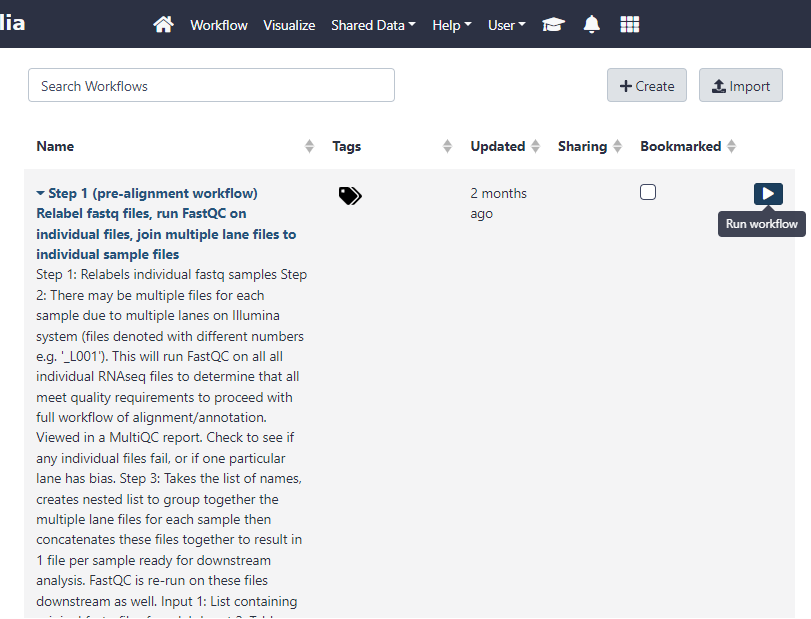
\includegraphics[width=1\linewidth]{images/image_run_workflow} 

}

\caption{Click the Run Workflow button}\label{fig:view-workflow}
\end{figure}

Once you've clicked `Run Workflow' it will let you select the files it should use and show all of the steps it will complete.
Select the appropriate files for 1 and 2. All other steps will not require user input.

\begin{figure}

{\centering 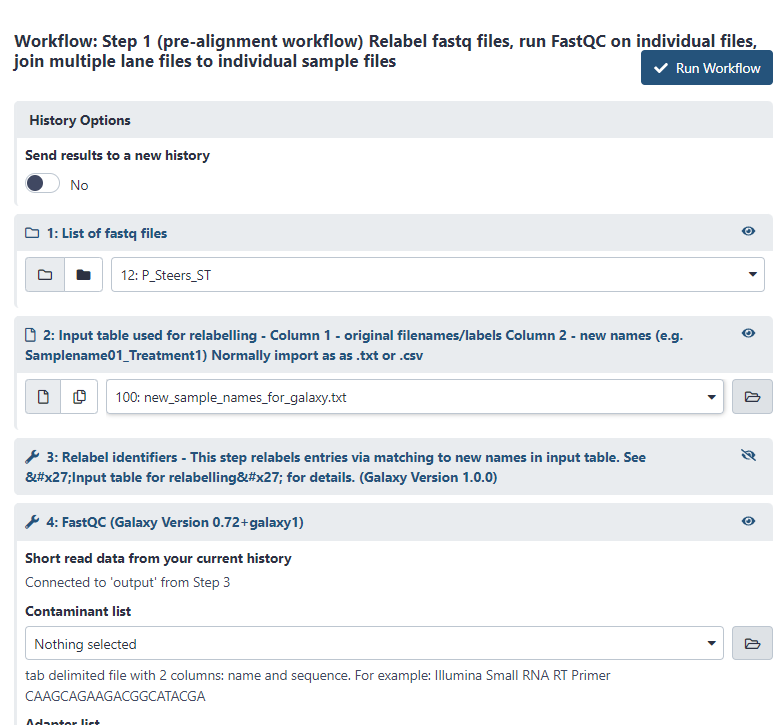
\includegraphics[width=1\linewidth]{images/image_run_workflow2} 

}

\caption{Select list of fastq files for number 1 and select the table of new names for number 2, then click 'Run Workflow'}\label{fig:run-workflow}
\end{figure}

This will invoke all steps and you will see them in the History.

\hypertarget{view-results}{%
\section{View results}\label{view-results}}

Once all steps are completed you will see the each part of the History has turned green.

\begin{figure}

{\centering 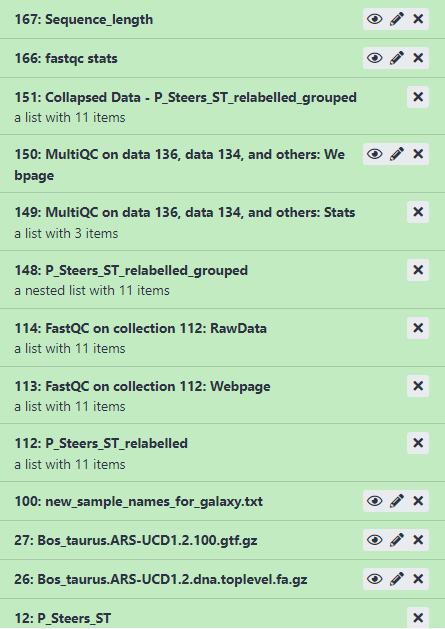
\includegraphics[width=6.18in]{images/image_history_after_step1} 

}

\caption{Example output in history after running first workflow}\label{fig:history-post-step1}
\end{figure}

The most interesting data will be found in the MultiQC webpage. It can be Viewed within galaxy but it may view better if downloaded and opened up in web browser.

\begin{figure}

{\centering 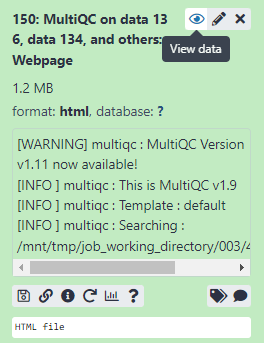
\includegraphics[width=3.67in]{images/image_view_multiQC} 

}

\caption{View the MultiQC webpage report}\label{fig:view-multiQC}
\end{figure}

There is plenty of help included in the report and it is worth noting that some sections will normally fail for RNAseq data. Although unlikely, it is also important to check if there are any major quality differences between lanes before proceeding (if multiple lanes exist).

\hypertarget{step-2}{%
\chapter{Step 2}\label{step-2}}

Step 2 completes multiple steps and reports output to one MultiQC report at the end, with various important outputs to the History.
The most useful output from this workflow for Differential Expression (DE) analysis is the table of counts with rows as gene names and columns as sample names.

The details of the pipeline are visible by following the workflow URL. In short, it uses trimmo

\hypertarget{import-workflow}{%
\section{Import workflow}\label{import-workflow}}

\url{https://usegalaxy.org.au/u/dave-innes/w/rna-seq-step-2}

\hypertarget{run-workflow-1}{%
\section{Run Workflow}\label{run-workflow-1}}

There are 4 required inputs to this workflow. Set it up as follows:

\begin{figure}

{\centering 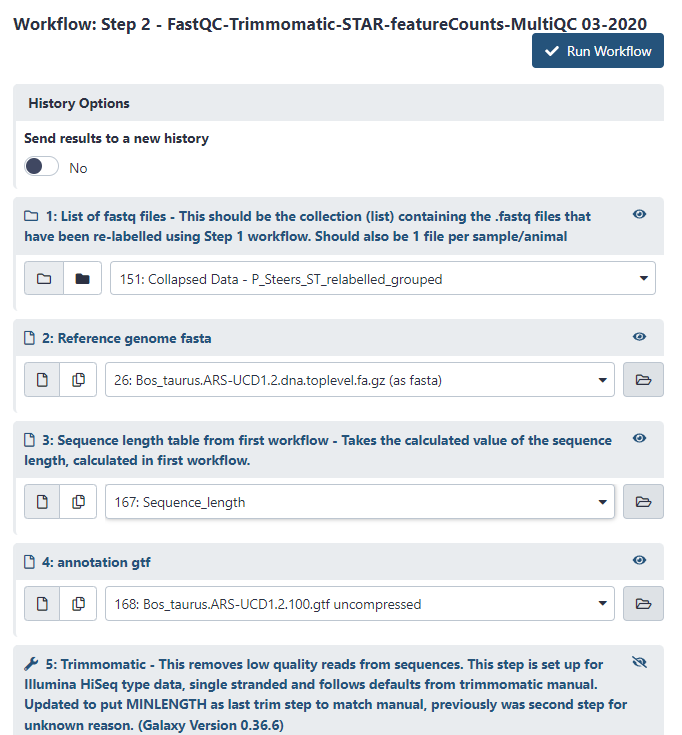
\includegraphics[width=1\linewidth]{images/image_step2} 

}

\caption{Setup Step 2 then press Run Workflow}\label{fig:run-workflow-step2}
\end{figure}

\textbf{This workflow will take a very long time to run. It runs on the Galaxy server and you can log in from any computer to see it's status. You're computer does not need to stay on. An email will also be sent to you once the last step is completed.}

\hypertarget{save-data}{%
\section{Save data}\label{save-data}}

Each analysis will require different outputs, but a simple DE analysis will normally only require the featureCounts output that is normally labelled as \texttt{featureCounts\_matrix.tabular}. Download this file. It can be previewed in Microsoft Excel by dragging and dropping into an active Excel window, however it is sometimes a large file and best handled in R or other similar software. Also be careful not to save changes if viewing in Excel as some gene names will be converted to date formats in excel and may introduce errors e.g.~\texttt{MARCH1} gene.

It is also recommended to save the MultiQC webpage and stats output. This is particularly useful for describing methods when writing up.

You may also want to view the specific alignments and therefore you will need the .bam files. See \url{https://software.broadinstitute.org/software/igv/BAM} for more information.

\hypertarget{inspect-report}{%
\section{Inspect Report}\label{inspect-report}}

It is important to view the MultiQC webpage and check that all output meets your quality requirements.

\hypertarget{multiple-lane-files}{%
\chapter{More notes on mutliple lane files}\label{multiple-lane-files}}

The output from Illumina sequencing is sometimes provided in multiple files, each corresponding to a `Lane' on the sequencer. It would be easier to ask the lab to provide the output as a single file, which can be computed using the \texttt{-\/-no-lane-splitting} option from Illumina's \texttt{bcl2fastq} program. However, it can also be handled in Galaxy.

\textbf{The following is a description of how to handle this manually. Please note that this is automated within Step 1 Workflow.}

If there are multiple files, it is best practice to run FastQC on each individual file, as there is a chance that one file could be corrupt or you may identify a bias for one particular `Lane'. If they are ok, then these files can be concatenated together before proceeding with all further steps. There are 2 workflows that will be used in Galaxy, with the first designed to work with each individual lane file and the second requiring 1 file per sample. This can be done by following these steps:

\begin{enumerate}
\def\labelenumi{\arabic{enumi}.}
\tightlist
\item
  `Apply Rule to Collection' tool
\item
  Input collection is the list with the re-labelled data
\item
  Press Edit button
\item
  There should be 1 column titled `A' with the names of the files (the re-labelled names set previously)
\end{enumerate}

\emph{Make new columns with grouping information:}

\begin{enumerate}
\def\labelenumi{\arabic{enumi}.}
\setcounter{enumi}{4}
\tightlist
\item
  Press +Column -\textgreater{} Using a regular expression
\item
  Select `Create column matching expression groups'
\item
  Paste the following code into the Regular Expression box: \texttt{(.*?)\_L(.*)}
\item
  Set the number of groups to 2
\item
  Press Apply
\end{enumerate}

\emph{Set columns as identifiers for grouping:}

\begin{enumerate}
\def\labelenumi{\arabic{enumi}.}
\setcounter{enumi}{9}
\tightlist
\item
  Press +Rules -\textgreater{} Add / Modify Column Definitions
\item
  Press +Add Definition -\textgreater{} List Identifiers
\item
  Select column B, then click on `Assign another column' and select C
\item
  Press Apply
\item
  Press Save, then Execute the job
\end{enumerate}

This outputs a nested list to the history. The number of items in the list should match the number of samples/animals, and then each sample in the list should contain the number of individual files (e.g.~2 or 3 files).

To then join this datasets together, the tool `Collapse Collection' will work in the background to be the same as using the `concatenate datasets tail-to-head' tool to concatenate the files individually. Although not clear in the tool's description, if it is provided a nested list, it will collapse the lowest level of groups together, in this case it is the Column C from above, which was the individual lanes. It should output a new list with the same number of files as the number of samples/animals. The names should be the names defined in Column B above: e.g.~2139\_Stage 2\_Fast:

\begin{enumerate}
\def\labelenumi{\arabic{enumi}.}
\tightlist
\item
  Open Collapse Collection tool
\item
  Choose to use a dataset collection, not an individual file
\item
  Select the nested list from above
\item
  Execute with all other default settings
\end{enumerate}

\end{document}
